\documentclass{article}
\newcommand{\beq}{\begin{equation}}
\newcommand{\eeq}{\end{equation}}
\newcommand{\ber}{\begin{eqnarray}}
\newcommand{\eer}{\end{eqnarray}}
\newcommand{\nn}{\nonumber}
\newcommand{\dd}[2]{\frac{d}{d{#2}}{(#1)} }
\newcommand{\pdd}[2]{\frac{\partial{#1}}{\partial{#2}}}
\usepackage{amsmath}
\usepackage{amsfonts}
\usepackage[hyphens]{url}
\usepackage{amssymb} 
\usepackage[utf8]{inputenc} 
%\usepackage[ngerman]{babel} 
\usepackage[T1]{fontenc}
\usepackage[margin=2.5cm]{geometry}
\usepackage{listings}
\usepackage{tikz}
\definecolor {processblue}{cmyk}{0.96,0,0,0}
\usetikzlibrary {positioning}
\usepackage{hyperref}
\begin{document}
\title{Backpropagation}
\author{Nachiket Gokhale}
\date{\today}
\maketitle
\section{Introduction}
Based on\\
\url{https://en.wikipedia.org/wiki/Automatic_differentiation}\\
\url{https://stats.stackexchange.com/questions/224140/step-by-step-example-of-reverse-mode-automatic-differentiation}\\
we study forward mode and reverse mode (backpropagation) differentiation.\\

Consider $f(x_1,x_2)= x_1x_2 + \sin(x_1)$. We want to compute $\pdd{f}{x_1}$ and $\pdd{f}{x_2}$. Analytically, we know

\beq
\pdd{f}{x_1} = x_2 + \cos(x_1) \qquad  \pdd{f}{x_2} = x_1 
\eeq

\section{Forward mode}
We need two separate passes for $\pdd{f}{x_1}$ and $\pdd{f}{x_2}$. For the first term we start with $x_1$ and go along all possible paths to $f$. For the first pass
\ber
\pdd{w_1}{x_1} &=& 1  \\
\pdd{w_4}{x_1} &=& \pdd{w_4}{w_1}\pdd{w_1}{x_1} = \cos(w_1) = \cos(x_1) \\
\pdd{w_3}{x_1} &=& \pdd{w_3}{w_1}\pdd{w_1}{x_1} = w_2 = x_2 \\
\pdd{w_5}{x_1} &=& \pdd{w_5}{w_4}\pdd{w_4}{x_1} + \pdd{w_5}{w_3}\pdd{w_3}{x_1} = (1)\cos(x_1) + (1)(x_2) = \cos(x_1) + x_2\\
\pdd{f}{x_1} &=&  \pdd{f}{w_5}\pdd{w_5}{x_1} = (1)(\cos(x_1) + x_2) = \cos(x_1) + x_2
\eer
For the second pass:
\ber
\pdd{w_2}{x_2} &=& 1 \\
\pdd{w_3}{x_2} &=& \pdd{w_3}{w_2}\pdd{w_2}{x_2} = w_1(1) = x_1 \\
\pdd{w_5}{x_2} &=& \pdd{w_5}{w_3}\pdd{w_3}{x_2} = (1)x_1 = x_1 \\
\pdd{f}{x_2} &=& \pdd{f}{w_5}\pdd{w_5}{x_2} = (1)(x_1) = x_1
\eer
Some efficiency may be obtained by calculating derivatives and storing them (which might almost become like reverse mode). But in general, we will need as many passes as the number of independent variables. 
\section{Reverse mode}
We start at the output and backtrack towards inputs over all possible paths.
\ber
\pdd{f}{w_5} &=& 1 \\ 
\pdd{f}{w_4} &=& \pdd{f}{w_5}\pdd{w_5}{w_4} = (1)(1) = 1 \\
\pdd{f}{w_3} &=&  \pdd{f}{w_5}\pdd{w_5}{w_3} = (1)(1) = 1
\eer
Now we need $\pdd{f}{w_1}$. Using our knowledge of the graph we can write
\ber
\pdd{f}{w_1} &=& \pdd{f}{w_4}\pdd{w_4}{w_1} + \pdd{f}{w_3}\pdd{w_3}{w_1} \\
             &=& (1)\cos(w_1) + (1)(w_2)
\eer
By using $w_1=x_1$ and $w_2=x_2$ we get
\ber
\pdd{f}{x_1} = \cos(x_1) + (1)(x_2)
\eer
Now we need $\pdd{f}{w_2}$. Using our knowledge of the graph we can write
\ber
\pdd{f}{w_2} = \pdd{f}{w_3}\pdd{w_3}{w_2} = (1)(w_1)
\eer
Using $w_2=x_2$ we can write
\ber
\pdd{f}{x_2} = x_1
\eer
Note that we have made only one pass backward through the graph. If we want to compute numerical values of the derivatives we will need one more pass forward through the graph to compute the numerical derivatives. 
\section{Computational graph}
\begin{figure}
  \centering
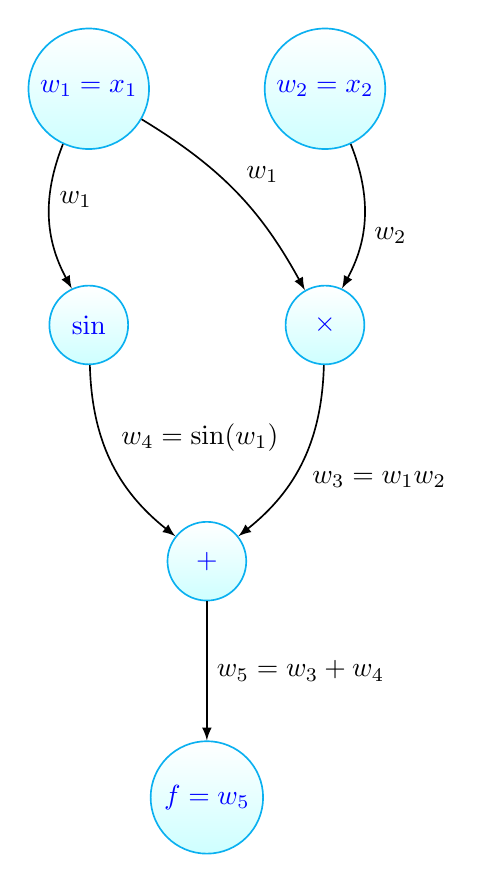
\begin{tikzpicture}[-latex ,auto ,node distance =3 cm and 3cm ,on grid ,
semithick ,
state/.style ={ circle ,top color =white , bottom color = processblue!20 ,
draw,processblue , text=blue , minimum width =1 cm}]
  \node[state](Input1){$w_1=x_1$};
  \node[state](Input2)[right = of Input1]{$w_2=x_2$};
  \node[state](sin)[below = of Input1]{$\sin$};
  \node[state](prod)[below = of Input2]{$\times$};
  \node[state](plus)[below left = 3 and 1.5 of prod]{$+$};
  \node[state](output)[below = 3.0 of plus]{$f=w_5$};
  \path (Input1) edge  [bend right = 25] node { $w_1$} (sin);
  \path (Input1) edge  [bend left = 15]  node { $w_1$} (prod);
  \path (Input2) edge  [bend left = 25] node { $w_2$} (prod);
  \path (sin) edge  [bend right = 25] node { $w_4=\sin(w_1)$} (plus);
  \path (prod) edge  [bend left = 25] node { $w_3=w_1w_2$} (plus);
  \path (plus) edge  [bend left = 0] node { $w_5=w_3+w_4$} (output);
\end{tikzpicture}
\caption{\label{fig:computationalgraph} Computational graph}
\end{figure}

\end{document}

